% !TeX TS-program = pdflatex
% !TeX encoding = UTF-8
% !TeX spellcheck = en_GB
% !TeX root = optarticle.tex
\documentclass[10pt,a4paper,fleqn]{article}
% -------------------------------- %
\usepackage{lmodern}
\usepackage[T1]{fontenc}
\usepackage{textcomp}
\usepackage[utf8]{inputenc}
\usepackage[UKenglish]{babel}
%\hyphenation{}
\usepackage{microtype}
\usepackage{indentfirst}
\usepackage[heightrounded]{geometry}
\usepackage{lipsum}
% -------------------------------- %
% Math
% -------------------------------- %
\usepackage{amsmath}
\usepackage{amssymb}
\usepackage{mathtools}
\usepackage{amsthm}
% -------------------------------- %
\newcommand{\numberset}{\mathbb}
%\newcommand{\N}{\numberset{N}}
\newcommand{\R}{\numberset{R}}
% -------------------------------- %
\renewcommand{\epsilon}{\varepsilon}
%\renewcommand{\theta}{\vartheta}
%\renewcommand{\rho}{\varrho}
%\renewcommand{\phi}{\varphi}
% -------------------------------- %
\DeclarePairedDelimiter{\abs}{\lvert}{\rvert}
\DeclarePairedDelimiter{\norma}{\lVert}{\rVert}
\DeclarePairedDelimiter{\set}{\{}{\}}
% -------------------------------- %
%\DeclareMathOperator{\sgn}{sgn}
%\DeclareMathOperator{\Realpart}{Re}
%\renewcommand{\Re}{\Realpart}
%\DeclareMathOperator*{\argmax}{arg\,max}
%\DeclareMathOperator*{\argmin}{arg\,min}
%\DeclareMathOperator{\Loss}{\mathit{L}}
\DeclareMathOperator{\loss}{\ell}
%\DeclareMathOperator{\regul}{\Omega}
\DeclareMathOperator*{\func}{\mathit{f}}
%\DeclareMathOperator*{\gradF}{\nabla\mathit{f}} % check if it works fine
%\DeclareMathOperator*{\hessF}{\nabla^2\mathit{f}}
%\DeclareMathOperator*{\Var}{Var}
%\DeclareMathOperator*{\bigO}{\mathcal{O}}
% -------------------------------- %
% Definitions
%\theoremstyle{definition}
%\newtheorem{defs}{Definition}
%\newtheorem{propts}{Property}
% Theorems
\theoremstyle{plain}
%\newtheorem{thm}{Theorem}
%\newtheorem{cor}[thm]{Corollary}
\newtheorem{prop}{Proposition}
%\newtheorem{lem}[thm]{Lemma}
% Remarks
%\theoremstyle{remark}
%\newtheorem{rmk}{Remark}
% -------------------------------- %
% Numbers
% -------------------------------- %
%\usepackage{siunitx}
%\sisetup{%
%	output-decimal-marker={,},group-separator={\,},%
%	round-mode=places%
%}
% -------------------------------- %
% Tikz and colors
% -------------------------------- %
%\usepackage{xcolor}
\usepackage{pgfplots} % + tikz
\pgfplotsset{/pgf/number format/use comma,compat=newest}
%%\usepackage{tikz} % + graphicx,keyval,xcolor
%%\definecolor{Maroon}{cmyk}{0,0.87,0.68,0.32}
%\definecolor{RoyalBlue}{cmyk}{1,0.50,0,0}
%%\definecolor{halfgray}{gray}{0.55}
%\definecolor{webgreen}{rgb}{0,0.5,0}
%\definecolor{webbrown}{rgb}{0.6,0,0}
\definecolor{lightergray}{gray}{0.99}
% -------------------------------- %
% Floating objects
% -------------------------------- %
%\usepackage{booktabs}
%\usepackage{tabularx}
%\usepackage{multirow}
\usepackage{subfig}
%\usepackage{wrapfig}
\usepackage{caption}
\captionsetup{format=hang,labelsep=colon,font={small,rm},labelfont={sf,bf}}
%\captionsetup[table]{skip=0.2\medskipamount,position=top}
\captionsetup[figure]{position=bottom}
\usepackage{flafter}
\usepackage[english,nospace]{varioref}
%\usepackage{enumitem}
% -------------------------------- %
% Code
% -------------------------------- %
\usepackage{listings}
%\renewcommand{\lstlistingname}{Algorithm}
% -------------------------------- %
%% R programming language
\definecolor{Rkwd}{rgb}{0.737,0.353,0.396}
\definecolor{Rparam}{rgb}{0.333,0.667,0.333}
\definecolor{Rnum}{rgb}{0.686,0.059,0.569}
\definecolor{Rstr}{rgb}{0.192,0.494,0.8}
\definecolor{Rcomm}{rgb}{0.678,0.584,0.686}
\lstdefinestyle{Rlang}{language=R,%
	keywordstyle=\color{Rkwd},basicstyle=\small\ttfamily,%
	commentstyle=\color{Rcomm}\ttfamily\em,%
	stringstyle=\color{Rstr}\rmfamily,%
	numbers=left,numberstyle=\tiny,stepnumber=1,numbersep=5pt,%
	showstringspaces=false,breaklines=true,frameround=ftff,%
	frame=lines,backgroundcolor=\color{lightergray},firstnumber=last%
	%	deletekeywords={}
}
% -------------------------------- %
% Python programming language
\lstdefinestyle{Pylang}{language=Python,%
	basicstyle=\small\ttfamily,%
	keywordstyle=,commentstyle=,stringstyle=,%
	numbers=left,numberstyle=\tiny,stepnumber=1,numbersep=5pt,%
	showstringspaces=false,breaklines=true,%
	frameround=ftff,frame=lines,%
	backgroundcolor=\color{lightergray},%
%	firstnumber=last,%
}
% -------------------------------- %
% Code output
\lstdefinestyle{output}{%
	basicstyle=\scriptsize\ttfamily,%
	showstringspaces=false,breaklines=true,frameround=ftff,%
	frame=lines,backgroundcolor=\color{lightergray},%
	%	deletekeywords={}
}
% -------------------------------- %
% Pseudo-code
\lstdefinestyle{simple}{%
	basicstyle=\small\ttfamily,%
	keywordstyle=\color{blue!20!red}\bfseries,%
	commentstyle=\color{darkgray},%
	stringstyle=\color{black},%
	numbers=left,numberstyle=\tiny,stepnumber=1,numbersep=5pt,%
	showstringspaces=false,breaklines=true,frameround=ftff,%
	frame=lines,backgroundcolor=\color{lightergray},%
	escapeinside={£!}{!£},%
	morekeywords={while,end,return,for,if},%
	%	comment={//},%
}
% -------------------------------- %

% -------------------------------- %
% My stuff
% -------------------------------- %
\newcommand{\myTitle}{Stochastic Gradient Descent with Momentum and Line Searches}
\newcommand{\mySubject}{Project work in Optimization Techniques for Machine Learning}
\newcommand{\myName}{David Nardi}
\newcommand{\myNameShort}{D. Nardi}
\newcommand{\mySummary}{MSc student in Artificial Intelligence, Univeristy of Florence}
\newcommand{\omissis}{[\textellipsis\unkern]}
\newcommand{\inToc}[1]%
	{\addcontentsline{toc}{section}{\texorpdfstring{\protect\numberline{}#1}{#1}}}
% -------------------------------- %
\title{\myTitle}
\author{\myName\\ \mySummary}
%\date{}
% -------------------------------- %
% Page styles
% -------------------------------- %
\usepackage{titleps}
\newpagestyle{main}{% oneside mainmatter
	\sethead[][][]%
	{\slshape\myNameShort}{}{\slshape\myTitle}%
	\setfoot[][][]%
	{}{\thepage}{}}
% -------------------------------- %
% Bibliography
% -------------------------------- %
% Activate bibliography when you are ready
%\usepackage[autostyle,italian=guillemets,babel]{csquotes}
%\usepackage[backend=biber,useprefix,style=ieee,backref,hyperref,defernumbers=true]{biblatex}
%\usepackage[backend=biber,useprefix,style=authoryear-comp,hyperref,defernumbers=true]{biblatex}
%\addbibresource{optarticle-bib.bib}
% -------------------------------- %
\usepackage{hyperref}
\hypersetup{%
%	colorlinks,urlcolor=webbrown,linkcolor=RoyalBlue,citecolor=webgreen,%
	linktocpage,pdfstartpage=1,bookmarksnumbered,bookmarksopen,bookmarksopenlevel=2,%
	pdftitle={\myTitle},pdfauthor={\myName},pdfsubject={\mySubject}%
}
% -------------------------------- %
\usepackage{showframe}
\begin{document}
\frenchspacing
% ************************************************************************************* %
% FRONTMATTER
% ************************************************************************************* %
\cleardoublepage
\pdfbookmark[1]{Title page}{fronte}
\maketitle

\begin{abstract}
\lipsum[1] % the one given with the assignment
\end{abstract}

\setcounter{tocdepth}{2}
\tableofcontents\cleardoublepage
\pagestyle{main}
% ************************************************************************************* %
% MAINMATTER %
% ************************************************************************************* %
% !TeX spellcheck = en_GB
% ***************************************************** %
\section{Introduction}\label{sc:intro}
% ***************************************************** %

% problem identification
% solutions

\subsection{Optimization problem}

\[
\min_{w\in\R^p}\func(w)=L(w)+\lambda\Omega(w)
\]

\begin{equation}\label{eq:opt-prob}
\min\sum_{i=1}^N\log\bigl(1+\exp(-y^{(i)}w^Tx^{(i)})\bigr)+\lambda\norma{w}^2
\end{equation}
where $i=\,\dots,N$ are the dataset indices, $y^{i}\in\set{-1,1}$ is the response variable corresponding to the negative or positive class, $x^{i}\in\R^p$ are dataset examples.

\[
\nabla\func(w)=X^Tr+2\lambda w,\quad r=-y^{(i)}\sigma(-y^{(i)}w^Tx^{(i)})
\]

\[
\nabla^2\func(w)=X^TDX+2\lambda I,\quad d_{ii}=\sigma(y^{(i)}w^Tx^{(i)})\sigma(-y^{(i)}w^Tx^{(i)})
\]

\begin{prop}
Problem~\eqref{eq:opt-prob} admits a unique optimal solution.
\end{prop}

\cleardoublepage

%\begin{figure}
%\centering
%\begin{tikzpicture}
%\begin{axis}[xlabel=$uv$,ylabel=$\ell$]
%\addplot[samples=200,blue,smooth] {ln(1+exp(-x))};
%\addplot[dotted] {0};
%\end{axis}
%\end{tikzpicture}
%\caption{Log-loss}
%\label{fig:log-loss}
%\end{figure}

\begin{figure}
\centering
\subfloat[][\emph{Log-loss}\label{subfig:log-loss}]%
{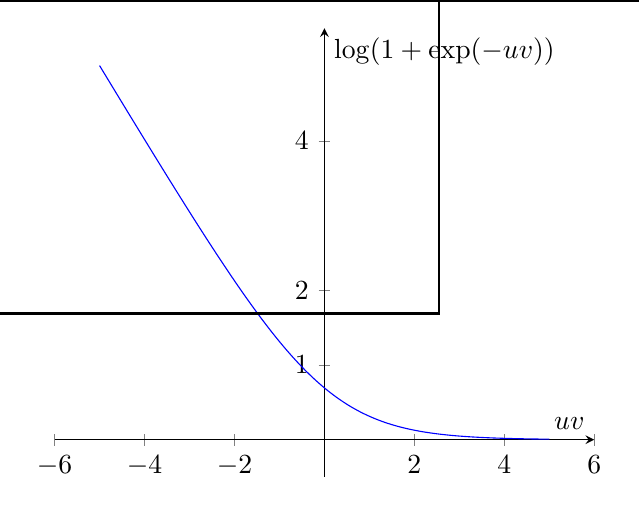
\begin{tikzpicture}
\begin{axis}[xlabel=$uv$,ylabel=$\log(1+\exp(-uv))$,ytick={1,2,4},axis lines=middle,enlargelimits]
\addplot[samples=200,blue,smooth] {ln(1+exp(-x))};
\end{axis}
\end{tikzpicture}} \\
\subfloat[][\emph{Sigmoid function}]%
{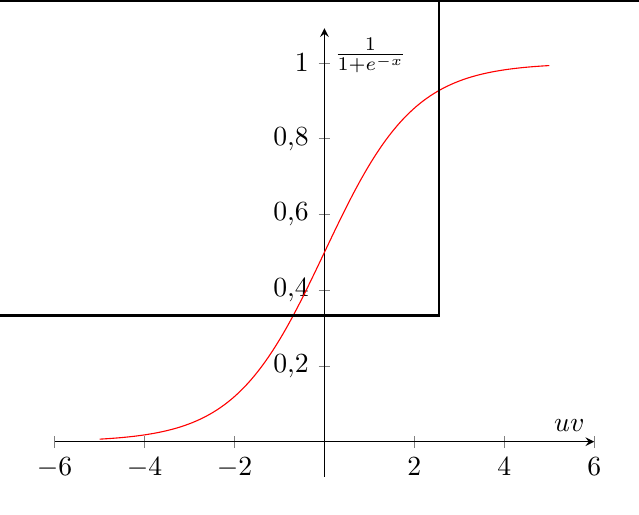
\begin{tikzpicture}
\begin{axis}[xlabel=$uv$,ylabel=$\frac{1}{1+e^{-x}}$,axis lines=middle,enlargelimits]
\addplot[samples=200,red,smooth] {1/(1+exp(-x))};
\end{axis}
\end{tikzpicture}}
\caption{Log-loss and sigmoid function plots}
\label{fig:log-sigma}
\end{figure}

%\begin{figure}
%	\centering
%	\subfloat[][\emph{First caption}\label{subfig:label1}]%
%	{\includegraphics[width=.45\textwidth]{}} \quad
%	\subfloat[][\emph{Second caption}\label{subfig:label2}]%
%	{\includegraphics[width=.45\textwidth]{}} \\
%	\subfloat[][\emph{Third caption}\label{subfig:label3}]%
%	{\includegraphics[width=.45\textwidth]{}} \quad
%	\subfloat[][\emph{Fourth caption}\label{subfig:label4}]%
%	{\includegraphics[width=.45\textwidth]{}} 
%	\caption[]{Global caption}
%	\label{fig:multifig}
%\end{figure}

\cleardoublepage

\begin{itemize}
\item $uv\gg0$: the example is labelled correctly
\item $uv\ll0$: the class assigned to the example is the wrong one
\end{itemize}

\begin{itemize}
\item the hessian matrix is positive defined $\forall w$, this means that the objective function, which is quadratic, is coercive and for the continuity that function admits global minimum, so $\func(w)$ has finite inferior limit
\item the hessian matrix being positive defined implies also that the objective function is strictly convex (on the other hand the loss function is just convex, due to its hessian matrix being positive semi-defined), this implies that if the global minimum exists, that solution is unique
\item a global minimum is a point that satisfy $\nabla\func(w^\ast)=0$, which is a sufficient condition implied by the convexity of the problem, see figure~\vref{subfig:log-loss}
\item the $\ell_2$ regularization implies that the objective function is strongly convex, this speeds up the convergence
\item further more we can assume that $\nabla\func(w)$ is Lipschitz-continuous with constant $L$
\end{itemize}

%\section{Theoretical results}

\cleardoublepage
\section{Mini-batch gradient descent variants}

\subsection{Fixed step-size}

\begin{lstlisting}[style=simple,title={Mini-batch Gradient Descent with fixed or decreasing step-size}]
dati £!$w^0\in\R^n$!£, £!$\func(w)=\sum_{i=1}^Nf_i(w)$!£, £!$k=0$!£ e £!$\set{\alpha_k}\mid\alpha_k=\alpha\vee\alpha_k=\frac{\alpha_0}{k+1}$!£
while (£!$\norma{\nabla\func(w^k)}>\epsilon$!£)
 shuffle £!$\set{1,\dots,N}$!£ in £!$N/M$!£ blocchi £!$B_1,\dots,B_{N/M}$!£ di dimensione £!$1<\abs{B_t}=M\ll N$!£
 £!$y_0=w^k$!£
 for £!$t=1,\dots,N/M$!£
  get mini-batch indices from £!$B_t$!£
  £!$y_t=y_{t-1}-\alpha_k\frac{1}{M}\sum_{j\in B_t}\nabla f_j(y_{t-1})$!£
 end for
 £!$w^{k+1}=y_{N/M}$!£
 £!$k=k+1$!£ fine epoca
end while
\end{lstlisting}

%\subsection{Decreasing step-size}

\subsection{Stochastic line search}

%compute true gradient approximation £!$\nabla f_{i_t}(w)$!£ with examples from £!$B_t$!£
\begin{lstlisting}[style=simple,title={Mini-batch Gradient Descent with Armijo line search}]
dati £!$w^0\in\R^n$!£, £!$\func(w)=\sum_{i=1}^Nf_i(w)$!£, £!$k=0$!£, £!$\gamma\in(0,1),\,\delta\in(0,1)$!£
while (£!$\norma{\nabla\func(w^k)}>\epsilon$!£)
 shuffle £!$\set{1,\dots,N}$!£ and split £!$B_1,\dots,B_{N/M}$!£ such that £!$1<\abs{B_t}=M\ll N$!£
 £!$y_0=w^k$!£
 for £!$t=1,\dots,N/M$!£
  get mini-batch indices £!$i_t$!£ from £!$B_t$!£
  approximate true gradient £!$\nabla f_{i_t}(w)=\frac{1}{M}\sum_{j\in B_t}\nabla f_j(y_{t-1})$!£
  £!$\alpha=\mathtt{reset()}$!£, £!$q=0$!£
  while (£!$f_{i_t}\bigl(y_{t-1}-\alpha\nabla f_{i_t}(w)\bigr)>f_{i_t}(y_{t-1})-\gamma\alpha\norma{\nabla f_{i_t}(y_{t-1})}^2$!£)
   £!$\alpha=\delta\alpha$!£
   £!$q=q+1$!£
  end while
  £!$\alpha_t=\alpha$!£
  £!$y_t=y_{t-1}-\alpha_t\nabla f_{i_t}(y_{t-1})$!£
 end for
 £!$w^{k+1}=y_{N/M}$!£
 £!$k=k+1$!£
end while
\end{lstlisting}

%\subsection{Fixed momentum term}

%\subsection{Corrected/restart momentum}


















% ************************************************************************************* %
% BACKMATTER %
% ************************************************************************************* %
%\phantomsection
%\inToc{\refname}
%\printbibliography
\end{document}
